% !TEX root = ../thesis_main.tex
%%%%%%%%%%%%%%%%%%%%%%%
\chapter{\pygbelspr: A computational biosensing application} \label{chap:pygbe-lspr}
\graphicspath{{pygbe_lspr_bio/figs/}}

\pygbelspr \cite{ClementiETal2017} is the python library for applications in 
nanoplasmonics. This application was added to the original \pygbe \cite{CooperETal2016} which
is used to study biomolecular electrostatics, and it extends \pygbe to nanoplasmonics, by treating 
localized surface plasmon resonance (LSPR) quasi-statically \cite{MayergoyzZhang2007}. In this chapter 
we show the verification of \pygbelspr as well as an application on LSPR biosensing. 

\section{Verification of \pygbe - Isolated silver nanoparticle } \label{sec:verification}

When we are in the long wavelength limit, we know that the electrostatic approximation 
applies and we can model the scattering of a small metallic sphere as a nanoparticle 
under a constant electric field (see Figure \ref{fig:sph_field}). This problem 
has an analytical solution and we use it to perform a grid-convergence analysis for 
the verification of the \pygbe solver.

In this section we show a verification study. We compare the numerical solution
obtained we \pygbe against an analytical solution available for spherical 
nanoparticles. 

The first analytical solution of the extinction cross section of spherical 
nanoparticles in vacuum, known as Mie-Theory, was presented by Gustav Mie in 1908
\cite{Mie1908}. This exact solution uses full electromagnetic theory, but in the 
long wavelength limit, electrostatics will lead us to the same solution 
\cite{BohrenHuffman1983} which is:

\begin{equation} \label{eq:Cext_analytical}
    C_\text{ext} = 4\pi a^3 k \operatorname{Im}\left(\frac{\epsilon_p/\epsilon_m -1}{\epsilon_p/\epsilon_m -2}\right)
\end{equation}

where $a$ is the radius of the nanosphere, $k$ the wave number, 
$\epsilon_p$ the dielectric constant od the nanoparticle, and $\epsilon_m$ the
dielectric constant of the host medium, in this case,  vacuum permittivity
($\epsilon_m = \epsilon_0$).  This formula, does not count for losses in the medium.
However, in 2007 Mishchenko presented a solution that counts for losses in
the host environment:

\begin{equation} \label{eq:Cext_analytical_lossy}
    C_\text{ext} = \frac{4\pi a^3}{k^\prime} \operatorname{Im}\left(k^2 \frac{\epsilon_p/\epsilon_m -1}{\epsilon_p/\epsilon_m -2}\right)
\end{equation}

where $k=k^\prime + k^{\prime\prime}i$. When the host medium is 
non-absorbing, $k$ is real ($k^{\prime\prime} = 0$ and $k=k^\prime$) and we 
recover \eqref{eq:Cext_analytical}. 

In the quasistatic limit (long wavelength approximation) the scattering 
of small particles can be explained using electrostatics, and model as
a nanosphere under a constant electric field (Figure \ref{fig:sph_field}) 
with analytical solution given by Eq. \eqref{eq:Cext_analytical_lossy}.

\begin{figure}%[h] %  figure placement: here, top, bottom, or page
    \centering
    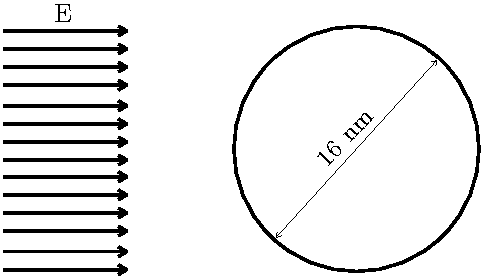
\includegraphics[width=0.55\textwidth]{sphere_field_8nm.pdf} 
    \caption{Spherical nanoparticle in a constant electric field.}
    \label{fig:sph_field}
\end{figure}

\subsection{Grid convergence analysis}\label{sub_sec:grid_conv_iso}

We perform a grid convergence analysis of \pygbe for a silver nanosphere 
of radius $r=8\,nm$ immersed in water, under a z-polarized electric field
of wavelength 380 nm and intensity of $-0.0037 e/(\text{\AA}^2 \, \epsilon_0)$.
For these conditions, the dielectric constant of water is
$1.7972 \, + \, 8.5048^{-09}i$ \cite{HaleQuerry1972} and for silver is
$-3.3877 \, + \, 0.1922i$ \cite{JohnsonChristy1972}. 
Table  \ref{table:quadparams1} shows the Gauss quadrature points used for each 
type of boundary element. We used a threshold parameter to define the near-singular
region of 0.5. This threshold defines the region of near singularity where 
semi-analytical technique is used. If $\sqrt{(2*Area)}/r > \text{threshold}$,
integration is done semi-analytically.
Table \ref{table:treeparams1} lists the parameters for the treecode and solver 
used in this convergence study.

\begin{table}%[h]
    \centering
    \caption{\label{table:quadparams1} Grid-convergence study: Gauss quadrature points; 
    $K$ and $K_{fine}$ are per element; $N_k $ is per element edge (semi-analytical integration). } 
    \begin{tabular}{l l}
    \hline%\toprule
     distant elements: & $K=4$ \\
     near-singular integrals:   & $ K_{fine}=37$ \\
     singular elements:  & $N_k =9$ \\
    \hline%\bottomrule
    \end{tabular}
\end{table}


\begin{table}%[h]
    \centering
    \caption{\label{table:treeparams1} Grid-convergence study: treecode and solver parameters.} 
    \begin{tabular}{l l}
    \hline%\toprule
    treecode order of expansion: & $P=15$\\
    MAC                          & $\theta=0.5$\\
    GMRES tolerance                    & $10^{-5}$\\
    \hline%\bottomrule
    \end{tabular}
\end{table}

Figure \ref{fig:conv_iso_sph} shows the results for the convergence study, with meshes of sizes 512, 2048, 
8192 and 32768 elements. The errors (Table \ref{table:err_iso_sph}) are computed against 
the analytical solution $C_{ext} = 1854.48$ nm$^2$ computed using Equation \eqref{eq:Cext_analytical_lossy}.
The dash line in Figure \ref{fig:conv_iso_sph} corresponds to a $1/N$ slope, and the observed order of 
convergence is $0.98$ which indicates that the meshes are correctly resolving the numerical solution with \pygbe.
The $1/N$ rate of convergence is consistent with convergence results in
previous work using \pygbe \cite{CooperBardhanBarba2013}. 

\begin{figure}%[h] %  figure placement: here, top, bottom, or page
    \centering
    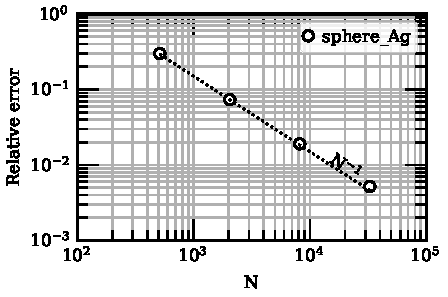
\includegraphics[width=0.85\textwidth]{convergence_sph_Ag_R8_w380.pdf} 
    \caption{Grid-convergence study for the extinction cross-section of a spherical silver
             nanoparticle, computed with \pygbe.}
    \label{fig:conv_iso_sph}
 \end{figure}
 
 
 \begin{table}%[h]
     \centering
     \caption{\label{table:err_iso_sph} Percentage error in the grid-convergence cases with an 
     isolated silver nanosphere.} 
     \begin{tabular}{c c}
     \hline%\toprule
     N & \% error \\
     \hline%\midrule
      $512$ & $29.86$ \\
      $2048$ & $7.33$ \\
      $8192$ & $1.9$ \\
      $32768$ & $0.52$ \\
     \hline%\bottomrule
     \end{tabular}
 \end{table}


\subsection{LSPR response of silver nanosphere}\label{sub_sec:lspr_silver_np}

To complement the verification test for the Localized Surface Plasmon Resonance (LSPR) implementation
on \pygbe, we computed the extinction cross section of the isolated silver sphere across multiple 
wavelengths. Figure \ref{fig:verif_sph} shows the results of comparing the simulations with the
analytical solution for a range of wavelengths from $[370-400]$ nm. The values of the dielectric 
for each wavelength were obtained by interpolation of experimental data 
\cite{HaleQuerry1972, JohnsonChristy1972}. To reproduce the interpolation study, we create
a Jupyter notebook and supporting code that can be find as part of the execution files
repro-package \cite{ClementiETal2018b}.
For this verification exercise we use a mesh of $N=32768$, and we relaxed some parameters 
compared to the ones used in the convergence analysis from section \ref{sub_sec:grid_conv_iso} 
that are shown in Tables \ref{table:quadparams2} and \ref{table:treeparams2}. The errors for each 
frequency are below $1\%$, and each runtime decrease by $12\times$.
Figure \ref{fig:verif_sph} exposes a good agreement between the analytical and simulation results, 
showing that \pygbe can accurately represent the mathematical model. Moreover, we can say that 
the level of accuracy is sufficient, given that the experimental uncertainty for the dielectric 
values for silver is in the order of $1\%$ \cite{JohnsonChristy1972}. 

\begin{figure}%[h] %  figure placement: here, top, bottom, or page
    \centering
    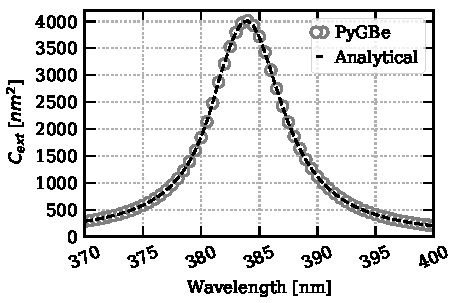
\includegraphics[width=0.85\textwidth]{silver_NP_verification.pdf} 
    \caption{Extinction cross-section as a function of wavelength for an $8$ nm
             silver sphere immersed in water. The peak in the values of 
             extinction cross-section corresponds to the plasmon resonance of the metallic 
             nanoparticle under the incoming electric field.}
    \label{fig:verif_sph}
 \end{figure}

\begin{table}%[h]
    \centering
    \caption{\label{table:quadparams2} Verification: Gauss quadrature points; 
    $K$ and $K_{fine}$ are per element; $N_k $ is per element edge (semi-analytical integration). } 
    \begin{tabular}{l l}
    \hline%\toprule
     distant elements: & $K=4$ \\
     near-singular integrals:   & $ K_{fine}=19$ \\
     singular elements:  & $N_k =9$ \\
    \hline%\bottomrule
    \end{tabular}
\end{table}


\begin{table}%[h]
    \centering
    \caption{\label{table:treeparams2} Verification: treecode and solver parameters.} 
    \begin{tabular}{l l}
    \hline%\toprule
    treecode order of expansion: & $P=6$\\
    MAC                                         & $\theta=0.5$\\
    GMRES tolerance                    & $10^{-3}$\\
    \hline%\bottomrule
    \end{tabular}
\end{table}

\section{LSPR response to Bovine Serum Albumin} \label{sec:lspr_response_bsa}

Localized surface plasmon resonance (LSPR) biosensors detect target molecules
by tracking frequency shifts in the plasmon resonance of metallic nanoparticles
in the presence of analytes \cite{WilletsVandyune2007}. The chapter presents the 
modeling of LSPR biosensors using \pygbe, and we show how our boundary elements approach is 
suitable to model this phenomenon. We compute the extinction cross section 
of a silver nanosphere with bovine serum albumin (BSA) proteins (PDB code: 4FS5,
BSA dimmer) in different locations around it. We placed two BSA dimers opposite to each other 
in three configurations ($\pm z$, $\pm y$, and $\pm x$), as shown by figures \ref{fig:display_z} and \ref{fig:display_xy}.
As a point of comparison, experiments by Teichroeb and co-workers
\cite{TeichroebETal2008} find a coverage of $2\times 10^{12} \quad \text{molecules}/cm^2$ or $3.3\times 10^{12} \quad \text{molecules}/cm^2$, 
with a gold sphere 15-nm in diameter. In that work, the molecular size reported is 5.5 nm$\times$5.5 nm$\times$9 nm, resulting in
a number of attached molecules between 4 and 6. The BSA molecule used in our work corresponds to a dimer, i.e., approximately 
double the size of that in Teichroeb et al.'s experiment. With two BSA dimers in the proximity of the sensor, 
the volume fractions in the near-by region are comparable.


\subsection{Grid convergence analysis} \label{sec:grid_conv_bsa}
We perform a grid convergence study to ensure that the meshes are correctly
resolving the numerical solutions. We performed the convergence analysis of
the system sketched in in Figure \ref{fig:analyte-sensor}. Given that we 
compute the extinction cross section by integrating over the sphere, we set 
a fixed mesh density for the protein and refined the mesh of the nanosphere 
(512, 2048, 8192, 32768 elements). For the protein, we found that a mesh with
two triangles per $\text{\AA}^2$ was fine enough for the convergence 
analysis, resulting in $N_{prot} = 98116$ elements.
We use the same conditions used in the grid convergence analysis of the 
isolated nanoparticle of section \ref{sub_sec:grid_conv_iso}, presented
in Tables \ref{table:quadparams1} and \ref{table:treeparams1}. The protein 
dielectric constant for a wavelength of 380 nm is $2.7514 + 0.2860i$, this  
value was computed using a functional relationship provided by Phan
 et al.~\cite{PhanETal2013}. The protein was located at a distance of 
 $d=$ 1 nm of the sphere along the z-axis, such that its dipole moment 
 was aligned with the y-axis. We show the errors in Figure  \ref{fig:err_sph-bsa} 
 and table \ref{table:err_sph-bsa} which were computed using the Richardson extrapolated
\ref{sec:rich_extrapolation} value of the extinction cross section $C_{ext}= 1778.73$ nm$^2$.

\begin{figure}%[h] %  figure placement: here, top, bottom, or page
    \centering
    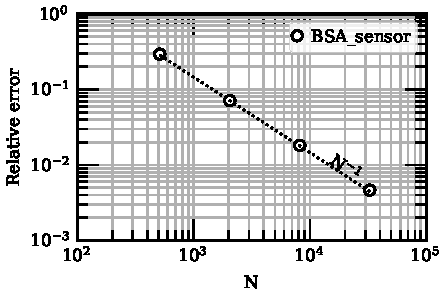
\includegraphics[width=0.85\textwidth]{convergence_bsa_sensor_R8_d1_w380.pdf} 
    \caption{Grid-convergence study of extinction cross-section of a spherical silver
             nanoparticle with a BSA protein at $d=1$ nm.}
    \label{fig:err_sph-bsa}
 \end{figure}

 \begin{table}%[h]
    \centering
    \caption{\label{table:err_sph-bsa} Estimated percentage error of the BSA-sensor 
    system (Fig.~\ref{fig:analyte-sensor}), with respect to the extrapolated value 
    (using Richardson extrapolation).} 
    \begin{tabular}{c c}
    \hline%\toprule
    N & \% error \\
    \hline%\midrule
     $512$ & $29.39$ \\
     $2048$ & $7.13$ \\
     $8192$ & $1.82$ \\
     $32768$ & $0.46$ \\
    \hline%\bottomrule
    \end{tabular}
\end{table}

The observed order of convergence is 0.99, and we can see in Figure
\ref{fig:err_sph-bsa} that the error decays with the number of boundary elements
at a rate of $1/N$, which is consistent with the verifications results showed
in Section \ref{sec:verification}. This shows that the numerical solutions computed
with \pygbe are correctly resolved by the meshes.

\subsection{Plasmon resonance frequency shifts} \label{sec:shift_bsa}

When a target molecule approaches the metallic nanoparticle, the resonance frequency
of this nanoparticle shifts. In this section, we computed the LSPR response as a
function of the wavelength in the presence of BSA protein. We optimized run times 
without compromising accuracy by using a relaxed set of parameters. For the protein
mesh density we used one element per $\text{\AA}^2$ ($N_{prot} = 45140$) and for the
sphere mesh we used $N_{sensor} = 32768$ elements. These calculations used the same
parameters from Tables \ref{table:quadparams2} and \ref{table:treeparams2}, which 
resulted in a percentage error below $1\%$, with respect to the Richardson-extrapolated
value. The run time for one frequency when two proteins are present, is approximately 
$15$ min using a NVIDIA Tesla K40c GPU.



\begin{center}
    \begin{figure} %  figure placement: here, top, bottom, or page
       \centering
       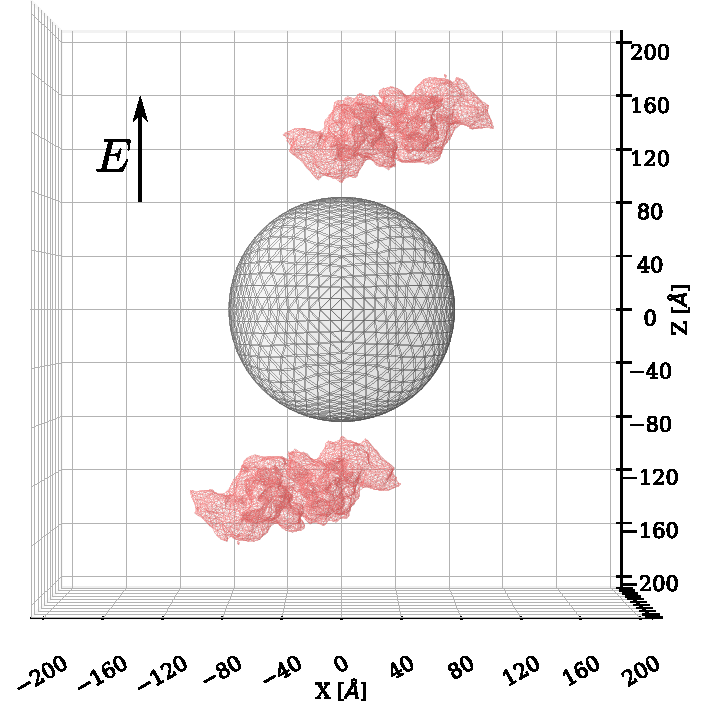
\includegraphics[width=0.85\textwidth]{2prot_1nm_z_R8nm.pdf} 
       \caption{Sensor protein display: BSA located at $\pm 1$ nm of the 
                nanoparticle in the $z$-direction.}
       \label{fig:display_z}
    \end{figure}
    \end{center}

Figure \ref{fig:display_z} shows a visualization of the meshes setup for these 
calculations, with two BSA proteins located at $d=1$ nm away from the spherical 
silver nanoparticle, along the $z$ axis. The position of the BSA molecule at $+z$ 
axis was the same used for the convergence analysis in section \ref{sec:grid_conv_bsa},
while the protein located in the $-z$ position is a 180$^\circ$ solid rotation 
about the $y$ axis, of the BSA in $+z$.  Figure \ref{fig:2pz_response} shows the results
of the calculations between 382 and 387 nm every $0.25$ nm, near the peak seen in Figure
\ref{fig:verif_sph}. In Figure \ref{fig:2pz_response} we have the variation of the 
extinction cross section with respect to wavelength for the isolated nanoparticle 
($d=\infty$) and with BSA proteins located at $d=1$ nm apart from the nanosphere. The
result shows a redshift ($0.5$ nm) in the resonance frequency due to the presence of 
the BSA analytes.

\begin{figure} %[h] %  figure placement: here, top, bottom, or page
    \centering
    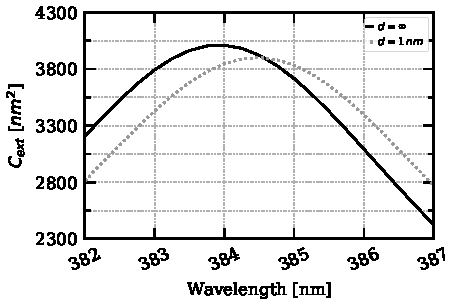
\includegraphics[width=0.85\textwidth]{2pz_R8nm.pdf} 
    \caption{Extinction cross-section as a function of wavelength for an $8$ nm
             silver sphere immersed in water with two BSA proteins placed 
             $\pm 1$ nm away from the surface in the $z$-direction, and at
             infinity (no protein).}
    \label{fig:2pz_response}
 \end{figure}

Figure \ref{fig:2pz_response} shows a redshift of the plasmon resonance frequency 
peak in the presence of two BSA proteins located at 1 nm along the $z$ axis. Experimental 
observations in the work of Tang, et al.~\cite{TangETal2010} revealed a redshift when 
BSA proteins in a solution are added to silver nanoparticles of approximately $17$ nm 
in diameter. They also observed a decrement of the peak amplitude, similarly to the 
effects we see with our model. Moreover, recent experiments \cite{PuETal2018} report 
resonance frequency between $380$ and $400$ nm for a silver nanosphere in the presence
of BSA proteins (check reference and its supplementary material), which is consistent with 
our results. Other experiments \cite{RaphaelETal2013} also report redshifts in the presence
of different proteins. The boundary element method approach that we implemented using 
electrostatic approximation is thus able to capture the characteristics of LSPR biosensors
based on resonance-frequency shift. 

We also study the effect of the location of the proteins, we performed the same 
calculations but now placing the BSA analytes along the $x$ and $y$ axis at $\pm 1$ nm,
as shown in Figure \ref{fig:display_xy}. We obtain these configurations by performing
a 90$^\circ$ solid rotation of the $z$-configuration (Figure \ref{fig:display_z})
along the $x$- and $y$-axis, respectively. 

 \begin{figure}
    \centering
    \subfloat{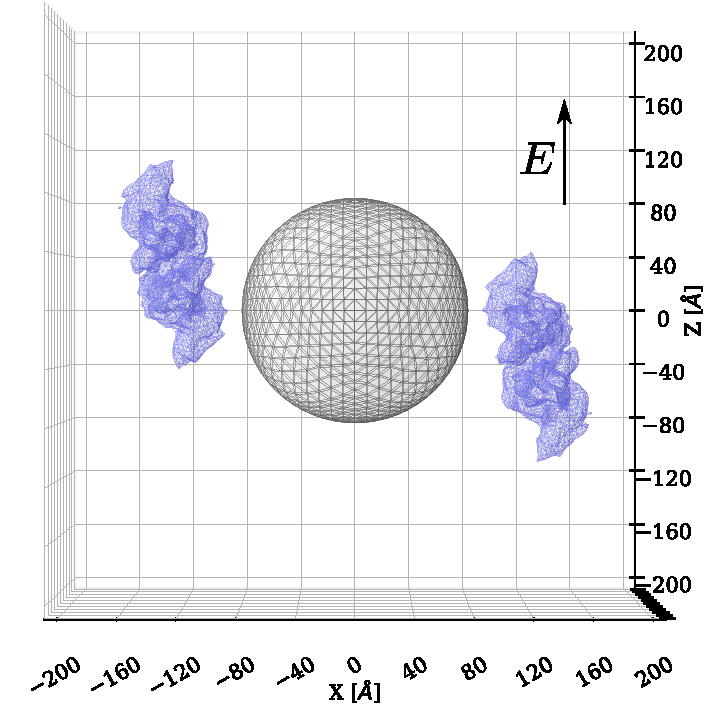
\includegraphics[width=0.65\textwidth]{2prot_1nm_x_R8nm.pdf}} \\
    \subfloat{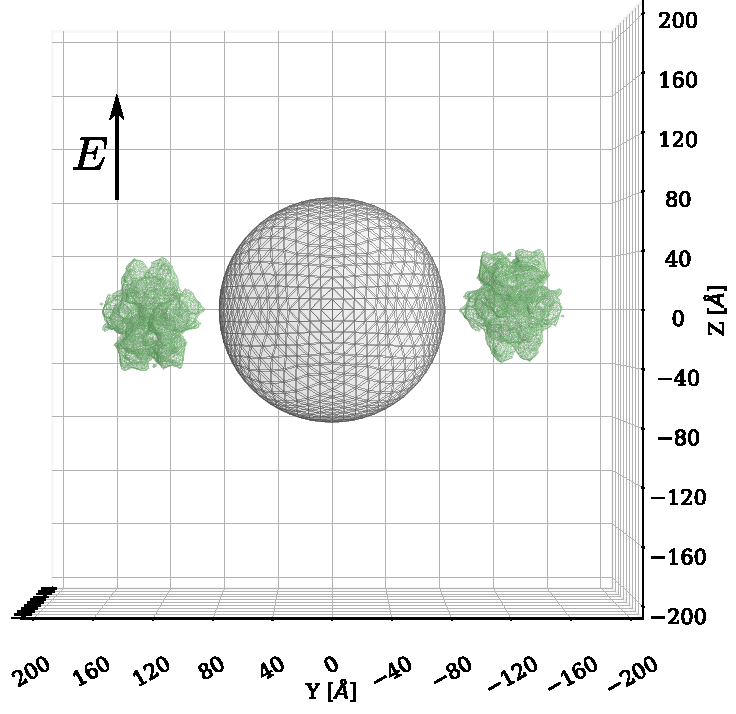
\includegraphics[width=0.65\textwidth]{2prot_1nm_y_R8nm.pdf}} 
     \caption{Sensor protein display: BSA located at $\pm 1$ nm of the nanoparticle in the
            $x$-direction (top) and $y$-direction (bottom).}
     \label{fig:display_xy}
 \end{figure}

 \begin{figure}%[t] %  figure placement: here, top, bottom, or page
    \centering
    \subfloat{\includegraphics[width=0.85\textwidth]{{2px_R8nm}.pdf}}\\
    \subfloat{\includegraphics[width=0.85\textwidth]{{2py_R8nm}.pdf}} 
    \caption{Extinction cross-section as a function of wavelength for an $8$-nm
             silver sphere immersed in water with two BSA proteins placed at
             $\pm 1 $ nm away from the surface in the $x$-direction (top) and
             $y$-direction (bottom), and at infinity (no protein).}
    \label{fig:2pxy_response}
 \end{figure}

Figure \ref{fig:display_xy} shows the configuration where the proteins are placed at a 
distance in the $x$ (top) or $y$ (bottom) direction, and Figure \ref{fig:2pxy_response} 
shows the  results for each configuration. For these setups where the 
 electric field is aligned with the $z$ axis, the LSPR response is negligible. The 
frequency shifts in Figure \ref{fig:2pxy_response} are smaller than the wavelength 
resolution ($<0.25$ nm). This finding is consistent with the free electrons oscillating
along the $z$ axis under a $z$-polarized electric field, and not in the $x$ and $y$ 
directions (see Figure \ref{fig:lspr}). The proteins have a marked effect when placed in the
$z$ direction, where they can interfere with the oscillation of the free electrons. 

\subsection{Sensitivity study} \label{sec:sensitivity}

On LSPR biosensors we refer to sensitivity to the relationship between the size of the 
resonance frequency shift and the number of analytes bound to the sensor (through the 
ligand). Experiments show that the distance between the protein and the nanoparticle 
affects the sensitivity of the sensor, to the point that targets placed 15 nm away 
from the surface are hardly detectable \cite{HaesETal2004}. This is a critical issue
considering that most common ligands, like antibodies, can be larger than 15 nm. In 
Figure \ref{fig:dist_response} we can see how the resonance peak varies with the distance 
at which the  analytes are located ($+z$ and $-z$). When $d=2$ nm we have a shift of 
$0.25$ nm while when the analytes are at $d=0.5$ nm the shift is $0.75$ nm. The parameters
used in these simulations remain the same as the ones used for the cases in Figures 
\ref{fig:2pz_response} and \ref{fig:2pxy_response}.

\begin{figure}%[h] %  figure placement: here, top, bottom, or page
   \centering
   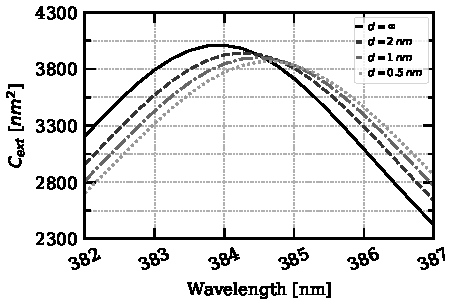
\includegraphics[width=0.85\textwidth]{2pz_lspr_response.pdf} 
   \caption{Extinction cross-section as a function of wavelength for an $8$-nm
            silver sphere immersed in water with two BSA proteins placed at
            $2$, $1$, and $0.5$ nm away from the surface in the 
            $z$-direction, and at infinity (no protein). The test case with
            $d=0.5$nm is close to the limit where quantum tunneling might happen. 
            Such effects are not captured by our classical model.}
   \label{fig:dist_response}
\end{figure}

As expected, Figure \ref{fig:dist_response} shows how the shift decreases as the BSA 
proteins move away from the nanoparticle, to the point that we only see a shift of 
$0.25$ nm when the analyte is $2$ nm away. This results shows the potential of \pygbe 
and the electrostatic approach to study biosensors sensitivity with distance. It's 
worth noting that quantum effects (e.g., tunneling) at $d=0.5$ nm are ignored with 
our classical approach. Even if this distance could be close to the quantum regime, 
there is evidence that classical theory is valid at this distance in similar systems
\cite{SavageETal2012, EstebanETal2012}

Even though there is evidence that techniques such as plasmon-enhanced Raman 
scattering are capable of detecting to the single-molecule limit 
\cite{ZhangZhangETal2013}, as far as we know there is no evidence of a purely
LSPR approach that can sense such low concentrations of proteins. Our 
computational results can unveil potential improvements that would enhance 
the sensitivity of LSPR biosensors, for example by using smaller ligands. 

There are not other LSPR simulations where the molecular details of the analyte 
are considered, that we are aware of. However, similar calculations can be 
performed with other open source softwares like BEM++ \cite{SmigajETal2015} and 
MATLAB toolbox MNPBEM \cite{HohenesterTrugler2012}. BEM++ also models the system
as a set of boundary integral equations, discretized in flat triangular panels, 
and it uses a Galerkin approach and algorithmic acceleration via hierarchical 
matrices. MNPBEM is another alternative software designed to simulate scattering
of metallic nanoparticles, which its BEM implementation is similar to \pygbe 
(centroid collocation with flat triangles) but with different acceleration scheme.
This MATLAB toolbox, similarly to BEM++, also relies on hierarchical matrices 
rather than a treecode, resulting in higher memory usage compared to our code, 
making it harder to simulate large analytes in detail. 
Commercial finite-element or finite-difference solvers can also be used for this
type of application, for example COMSOL. However, these volumetric approaches 
struggle to correctly impose the zero boundary condition at infinity, which is
exactly met for BEM.  

\section{Reproducibility and data management} \label{sec:repro_lspr}

All the results of this chapter have been published in the journal 
Physical Review E \cite{ClementiETal2019} and can be reproduced or replicated. \pygbe is openly developed and 
shared under the BSD3-clause license via its repository at \url{https://github.com/barbagroup/pygbe}.

All results of this chapter were obtained on a lab workstation, built from parts. Hardware specifications are as follows:

\begin{itemize}
  \item CPU: Intel Core i7-5930K Haswell-E 6-Core 3.5GHz LGA 2011-v3
  \item RAM: G.SKILL Ripjaws 4 series 32GB (4 x 8GB)
  \item GPU: Nvidia Tesla K40c (with 12 GB memory)
\end{itemize}

We release all of the data and scripts needed to run the calculations reported in this chapter, 
as well as the post-processing scripts to reproduce the figures. 
All the input files necessary to reproduce the computations are available in a Zenodo data set \cite{ClementiETal2018a}. 
Each folder contains the geometry files and charges files when applicable (.pqr), configuration files and parameter files.
We provide the scripts and any additional file needed to run \pygbe to re-generate every result in this chapter, in a 
separate Zenodo deposit \cite{ClementiETal2018b}. The execution of these scripts will generate the user's own version of the data needed to re-create 
the figures of this chapter (For more details, the reader can consult a \texttt{README} file in the Zenodo archive).
Finally we provide \emph{Reproducibility packages} deposited on Figshare to reproduce the figures in this chapter, which include 
figures, plotting scripts and Jupyter notebooks that organize and re-create the results 
\cite{ClementiETal2018c,ClementiETal2018d,ClementiETal2018e,ClementiETal2018f}.
